\chapter{Introduction}\label{sec:intro}
\begin{flushright}{\slshape    
The most important contribution of management in the 20th century\\
was to increase manual worker productivity fifty-fold.\\
The most important contribution of management in the 21st century\\
will be to increase knowledge worker productivity\\
— hopefully by the same percentage} \\ \medskip
--- Peter Drucker~\cite{drucker1999}
\end{flushright}

When Peter Drucker became aware that the automation of manual labour was progressing faster than that of knowledge work, he said these words at the end of the $20^{th}$ century in 1999. Between both types of work lies a pronounced difference: The course of manual work is determined by physical laws, while the course of knowledge work requires one to "think for a living" and allows for flexible execution of the work. This flexibility incurs another dimension: many decisions, as small as they may be, need to be made by the knowledge worker based upon information.

Now, 20 years later, numerous knowledge repositories and assistance systems for knowledge workers exist, helping make decisions more informed and faster. These assistance systems also often log the course of a case until its completion. Instances of a process are henceforth referred to as cases.\\

This work makes use of these logs and presents a step towards actively assisting the knowledge worker by predicting the activity which would usually be executed next in the context of a case's execution. This prediction could then be processed further in a process guidance system for knowledge workers. In this work, these predictions are derived from a special type of neural network.\\

\begin{figure}
    \centering
    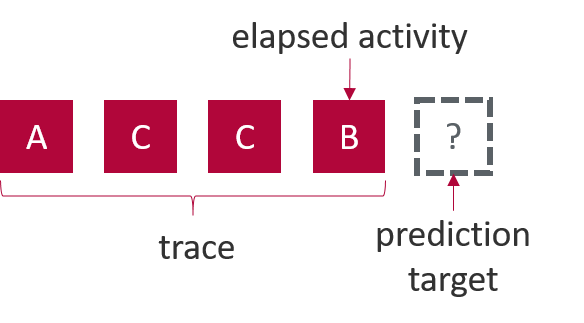
\includegraphics[width=\textwidth]{gfx/next-activity.png}
    \caption{Predicting the next activity, TODO replace}
    \label{fig:next-activity-prediction}
\end{figure}

The application of Predictive Analytics in Process Science is fairly new, and is now commonly referred to as Predictive Process Monitoring (see \autoref{chap:background}), although no formal definition exists yet. As it is a new domain, only a small number of publications have addressed the next-activity prediction problem. Much more work exists on typical prediction problems for less knowledge-driven business processes, where models can be enforced: prediction of predicate conformance or completion time (see \autoref{fig:next-activity-prediction}), to name two. Furthermore, the fact that no domain-specific benchmarking dataset for this kind of problem exists yet, makes the few existing publications hard to compare, as they work on different data. There is however a tendency to make use of the datasets of the Business Process Intelligence Competition (BPIC)~\cite{BPIC2011, BPIC2012, BPIC2017}, which publishes a new dataset for every year. And lastly, the next-activity prediction problem has not been related to similar problems in domains in which more work has already been done (see \autoref{chap:related-work}.\\

This thesis addresses these facts by proposing a revised prediction model that was inspired by predictive models applied in the area of Natural Language Processing (NLP). This approach is tested on the datasets of BPIC2011 and BPIC2012 and compared to two implementations taken from the following papers, thus allowing for a direct comparison (see \autoref{chap:contribution}):

\begin{enumerate}
    \item \textit{A Deep Learning Approach for Predicting Process Behaviour at Runtime} by Evermann et al.~\cite{evermann2016} \item\textit{Deep Learning Process Prediction with Discrete and Continuous Data Features} by Schönig et al.~\cite{schoenig2018}.
\end{enumerate}

Over the course of the reverse-engineering of the comparison models and the subsequent evaluation (see \autoref{chap:evaluation}), widely divergent understandings and approaches with regard to the structure of sequential data input for neural networks were noted. To contribute to a better understanding, a comparison of the perceived possibilities was incorporated into the contribution.

The findings of this thesis can also be found summarized in the last chapter of this document, \autoref{chap:conclusion}.

\newpage
\section{Research questions}\label{sec:intro:objective}
In this thesis, we want to investigate the applicability of a NLP next-element prediction approach on process event logs. In direct comparison to alternative approaches, performance statements shall be made as well as a suggestion for input data structuring. This leads to the two following research questions:

\begin{enumerate}
    \item Does a NLP-inspired approach provide better prediction accuracy over state-of-the-art approaches?
    \begin{enumerate}
        \item If so, which engineered feature helps in doing so?
        \item Does the engineered feature improve the other approaches as well?
    \end{enumerate}
    \item What is the preferable method for training a neural network with sequential data of variable length?
\end{enumerate}